%%% This Beamer example was created by LianTze Lim, April 2017.

%%%% This is a VERY simple and minimalistic beamer theme,
%%%% even reminiscent of marker pens on transparencies!
%%%% It mimics the look of the "seminar" package, which
%%%% can only be used with plain TeX.
%%%% There are also some comments and example to show how
%%%% to customise various elements, e.g. the font and colours.

\documentclass[12pt]{beamer}
%% If you'd like the default font size to be even larger, use 14pt or 17pt; these are supported by Beamer.

\graphicspath{{Figures/}{Figures}}

%%%%%%%%%%%%%%%%%%%%%%%%%%%%%%%%%%%%%%%%%
% These lines should usually go into a .sty file,
% but I'll leave them here so that it's easier to
% see how to customise a Beamer theme.
% Remember, the Beamer manual is your friend!!
% http://texdoc.net/pkg/beamer
%
%% So if your re-definitions have a @ somewhere, you
%% _MUST_ put a \makeatletter before these lines and then
%% \makeatother after them. This trick can only be done
%% in the preamble! BUT if you're doing these re-definitions
%% in a .sty file (so that you \usepackage it later), you
%% don't need the \makeatletter and \makeatother.
\makeatletter

%% Set the left and right margins
\setbeamersize{text margin left=1em,text margin right=1em}

%% FONTS
\setbeamerfont{title}{series=\bfseries,size=\LARGE}
\setbeamerfont{subtitle}{series=\bfseries,size=\Large}
\setbeamerfont{frametitle}{series=\bfseries,size=\small}
\setbeamerfont{block title}{series=\bfseries,size=\normalsize}
\setbeamerfont{footline}{size=\small}

%% COLOURS
%% If you'd like everything to have the same colour
\usebeamercolor{structure}
\setbeamercolor{normal text}{fg=structure.fg}

%% Add a line after the frametitle
\addtobeamertemplate{frametitle}{}{\vspace*{-1ex}\rule{\textwidth}{1pt}}

%% Use circular discs as itemized list markers;
%% there's an existing option in Beamer for it so I'll use it
\setbeamertemplate{itemize items}[circle]

%% Remove default navigation symbols (We'll add the ones we need in the footline
\setbeamertemplate{navigation symbols}{}


%% And before the footline... actually we'd like to re-define
%% the footline
\setbeamertemplate{footline}{%
   %% Beamer headlines and footlines are always full-paperwidth, so if you want the horizontal line to
   %% not span it entirely you'll need to do a bit of arithmetic
   \centering
   \begin{minipage}{\dimexpr\paperwidth-\beamer@leftmargin-\beamer@rightmargin\relax}
   \centering
   \rule{\linewidth}{1pt}\vskip2pt
   \usebeamerfont{footline}%
   \usebeamercolor{footline}%
   %% The frame number smack in the middle
   \hfill\insertframenumber/\inserttotalframenumber
   \hfill%
   %% ONLY the navigation symbols we want at the far right.
   %% We use an \llap so that it takes up zero width, and doesn't throw the page number off-centre!
   \llap{\insertframenavigationsymbol\insertbackfindforwardnavigationsymbol}\par
   \end{minipage}\vskip2pt
}

\setbeamercolor{block title alerted}{fg=white,bg=brown}

\makeatother
%%%% END STYLE CUSTOMISATION %%%%%%%%%%%%

\usepackage[english]{babel}
\usepackage[latin1]{inputenc}
\usepackage[T1]{fontenc}
\usepackage{graphicx}

\usepackage{subcaption}

\usepackage{times}

\usepackage{graphics}
%\usepackage[draft]{graphics}

\usepackage{xspace}
\usepackage{amsmath}
\usepackage{bm}
\usepackage{pgfpages}
\usepackage{fancybox}
\usepackage{threeparttable}
\usepackage{bbding}
\usepackage{verbatim}
\usepackage{booktabs}

\usepackage{natbib}
\bibpunct{(}{)}{;}{a}{}{,}

\newcommand{\pkg}[1]{{\normalfont\fontseries{b}\selectfont #1}}
\let\proglang=\textsf
\let\code=\texttt

\newcommand{\btheta}{ \mbox{\boldmath $\theta$}}
\newcommand{\bbeta}{ \mbox{\boldmath $\beta$}}
\newcommand{\balpha}{ \mbox{\boldmath $\alpha$}}
\newcommand{\by}{ \mbox{\bf y}}
\newcommand{\bY}{ \mbox{\bf Y}}
\newcommand{\bX}{ \mbox{\bf X}}
\newcommand{\bH}{ \mbox{\bf H}}
\newcommand{\bI}{ \mbox{\bf I}}


\title{Spatial autocorrelation and neighbourhood structure}
\subtitle{}
\author{Bayesian modelling for spatial and spatio-temporal data}
\institute{MSc in Epidemiology}
\date{Week 6}


\begin{document}

\begin{frame}[t]
  \titlepage
\end{frame}

\begin{frame}
\frametitle{Recap on areal data}
\begin{itemize} \setlength\itemsep{\fill}
\item  The data are referenced at an aggregate level and are often defined by administrative boundaries (states, counties, districts etc.).
\item  Areal units are generally irregular geographic areas and in spatial epidemiology we have a collection of areal units.
\item  We care about how areal units connect to each other and we use neighbour information to define spatial relationships.
\item  In what follows, we will consider a study region to be divided into $N$ disjunctive areas indexed by $i$, for $i=1,\dots,N$.
\end{itemize}
\end{frame}


\begin{frame}
\frametitle{Spatial Autocorrelation}
\begin{itemize} \setlength\itemsep{\fill}
\item A key insight is that observations in space cannot in general be assumed to be mutually independent, and that observations that are close to each other are likely to be similar (remember Waldo Tober's first law of geography).
\item  This spatial patterning, or \alert{spatial autocorrelation}, may be treated as useful information about unobserved influences.
\item  Formally, spatial autocorrelation measures the correlation of a variable with \emph{itself} through space. If $Z_i$ is the attribute $Z$ observed at location $i$, then the term spatial autocorrelation refers to the correlation between $Z_i$ and $Z_j$.
\item In other words, it quantifies the degree of which observations, at spatial locations, are similar to nearby observations.
  \end{itemize}
\end{frame}

%\begin{frame}
%\frametitle{Spatial Autocorrelation [2]}
%\begin{itemize} \setlength\itemsep{\fill}
%\item  Every real map presents areas with some relatively higher values clustered in some parts of the map. Other parts present relatively lower valued areas.
% \item  We also meet much \emph{noise}: sub-regions with high and low values mixed randomly without any spatially structured pattern.
%\item It is no easy just visually determine whether values are spatially clustered.
%  \end{itemize}
%\end{frame}


\begin{frame}
\frametitle{Detecting spatial autocorrelation}
\begin{itemize} \setlength\itemsep{\fill}
\item  The detection of spatial autocorrelation is useful in spatial analysis for identifying underlying data structures, the degree of spatial randomness, or clustering in the data.
\item  Tests of spatial autocorrelation examine whether the observed value of a variable at one location is independent of values of that variable at neighbouring locations.
\end{itemize}
\end{frame}

\begin{frame}
\begin{itemize} \setlength\itemsep{\fill}
\item  \alert{Positive spatial autocorrelation} indicates that similar values appear close to each other, or cluster, in space (figure a)
\item  \alert{Negative spatial autocorrelation} indicates that neighboring values are dissimilar or, equivalently, that similar values are dispersed (figure b)
\item  \alert{Null spatial autocorrelation} indicates that the spatial pattern is random (figure c)
\end{itemize}
\begin{figure}
  \centering
  \begin{subfigure}[b]{0.26\linewidth}
    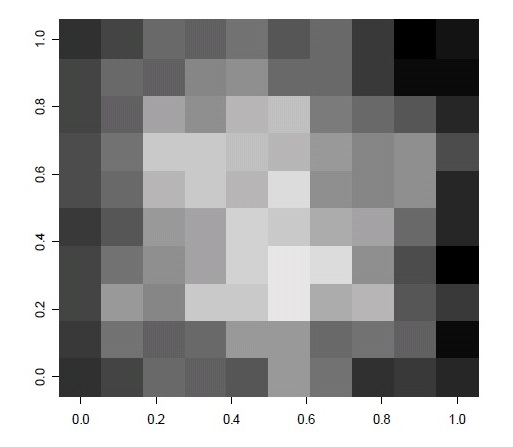
\includegraphics[width=\linewidth]{Pos_SpatCorr.jpg}
    \caption{}
  \end{subfigure}
  \begin{subfigure}[b]{0.24\linewidth}
    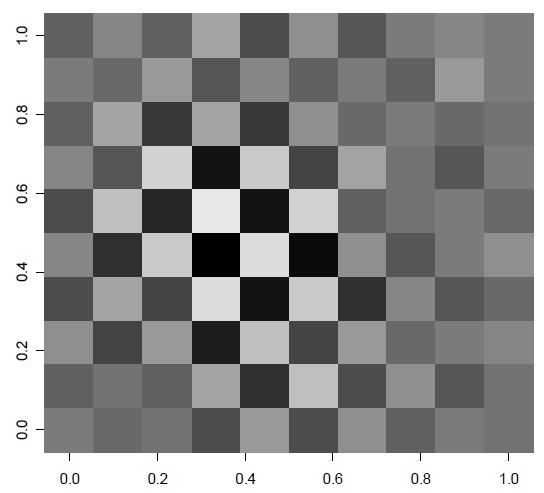
\includegraphics[width=\linewidth]{Neg_SpatCorr.jpg}
     \caption{}
  \end{subfigure}
  \begin{subfigure}[b]{0.24\linewidth}
    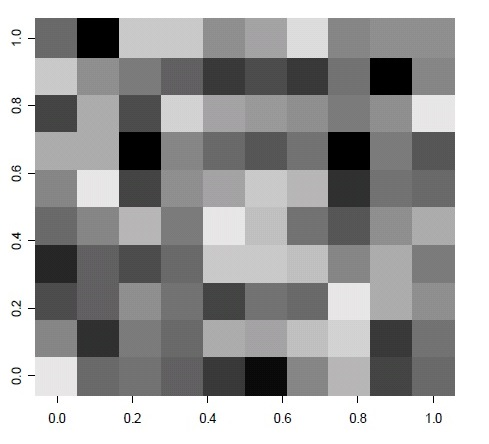
\includegraphics[width=\linewidth]{Null_SpatCorr.jpg}
     \caption{}
  \end{subfigure}
\end{figure}




\end{frame}

%%%%%%%%%%%%%%%%%%%%%%%%%%%%%%%%%%%%%%%%%%%%%%%%%%%%%%%%%%%%%%%%%%%%%
\begin{frame}
\frametitle{Spatial neighbours [1]}
\begin{itemize} \setlength\itemsep{\fill}
\item Key to analyse lattice (or regional) structures is the concept of \emph{spatial connectivity} or \emph{spatial proximity}.
\item Let $i$ and $j$ index two members of the lattice (i.e. two locations such as two countries, or two districts etc.).
\item With each pair of sites, we associate a \alert{weight $w_{ij}$}, so that the spatial weights express the neighbour structure between the observations.
\end{itemize}
\end{frame}

\begin{frame}
\frametitle{Spatial neighbours [2]}
\begin{itemize} \setlength\itemsep{\fill}
\item Now, let $N$ be the total number of areal units.
\item The spatial relationship between the areas is represented as an adjacency matrix $\mathbf{W}$ with dimensions $N \times N$, where the entries $w_{ij}$ of the matrix are the spatial weights:
 \begin{equation*}
\mathbf{W} =
\begin{bmatrix}
w_{11} & w_{12} & \cdots & w_{1N} \\
w_{21} & w_{22} & \cdots & w_{2N} \\
\vdots  & \vdots  & \ddots & \vdots \\
w_{N1} & w_{N2} & \cdots & w_{NN}
\end{bmatrix}
\end{equation*}
\begin{itemize} \setlength\itemsep{\fill}
\item In its simple form, $w_{ij}=1$ if areas $i$ and $j$ are adjacent, 0 otherwise\footnotemark.
\item The diagonal elements of $\mathbf{W}$ are zero, that is $w_{ii}=0$.
\end{itemize}
\end{itemize}
\footnotetext[1]{The binary (0/1) matrix $\mathbf{W}$ based on contiguity is sometime referred to as the first order contiguity weights because it define the immediate neighbours.}
\end{frame}

\begin{frame}
\frametitle{Weights based on contiguity}
Operationally, we can distinguish between a \textcolor{cyan}{rook} (A) and a \textcolor{cyan}{queen} (B) criterion of contiguity between areas (in analogy to the moves allowed for the such-named pieces on a chess board):
\begin{columns}
\column{0.5\textwidth}
\begin{figure}
  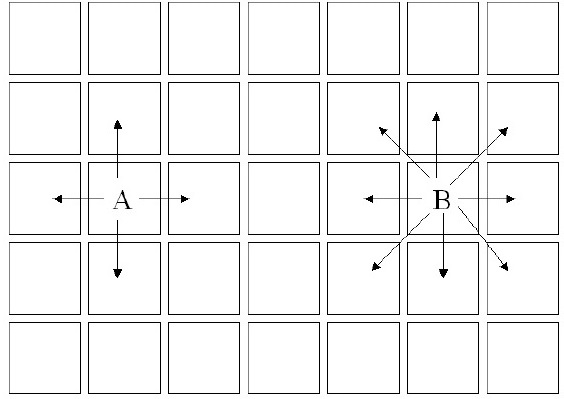
\includegraphics[width=1.7in]{Weights.jpg}
\end{figure}
\column{0.5\textwidth}
\small{The \textcolor{cyan}{rook} criterion defines neighbours by the existence of a common edge between two spatial units.\\ The \textcolor{cyan}{queen} criterion defines neighbours as spatial units sharing a common edge or a common vertex}.
\end{columns}
\end{frame}

\begin{frame}
\frametitle{Weights based on geographical distance [1]}
\begin{itemize} \setlength\itemsep{\fill}
\item Other ways of measuring the \emph{closeness} between areas are based on the distance $d_{ij}$ (Euclidean, Manhattan or other metrics) between units $i$ and $j$ (where $i\neq j$).
\item Distance can be taken between geometric centroid of each polygon:
\begin{itemize} \setlength\itemsep{\fill}
\item $w_{ij}=d{ij}^{-1} $, inverse distance between the centroids of areas $i$ and $j$
\item $w_{ij}=d^{-\gamma}_{ij}$, inverse distance raised to the power $\gamma >0$
\item $w_{ij}=\exp(-\gamma d_{ij})$, negative exponential, with $\gamma >0$
\end{itemize}
\item The diagonal elements on $\mathbf{W}$ are equal to zero. The off-diagonal elements of $\mathbf{W}$, will be non-zero, unless we impose a thresholds.
\end{itemize}
\end{frame}

\begin{frame}
\frametitle{Weights based on geographical distance [2]}
Commonly used thresholds are:
\begin{itemize} \setlength\itemsep{\fill}
\item absolute distance threshold: if $d_{ij}\geq x$ (i.e. the centroids of areas $i$ and $j$ are within a certain distance of each other), otherwise $w_{ij}=0$;
\item based on $k$ nearest neighbours: only the $k$ nearest neighbours of unit $i$ are non-zero (in this case the weights will not be symmetric\footnotemark).
\end{itemize}
\footnotetext[2]{The matrix $\mathbf{W}$ is symmetric when $w_{ij}=w_{ji}$}
\end{frame}

\begin{frame}
\frametitle{Spatial neighbours in R}
In R, we need to define:
\begin{itemize} \setlength\itemsep{\fill}
  \item Neighbour connectivity (who is neighbour?)
  \item Neighbor weights (how much does the neighbour matter?)
\end{itemize}
To do so, we can work with the package \texttt{spdep} and we use:
\begin{itemize} \setlength\itemsep{\fill}
\item the function \texttt{poly2nb} to define neighbour connectivity according to rook or queen criterion (contiguity neighbours)
\item the functions \texttt{knn2nb} and \texttt{dnearneigh} to define neighbour connectivity according to distance-based neighbours
\item the function \texttt{nb2listw} to define spatial weights for neighbours lists (while \texttt{nb2mat} defines spatial weights matrices for neighbours lists)
\end{itemize}
    \vspace{10pt}
\tiny{For further details, see Roger Bivand's contribution \url{https://r-spatial.github.io/spdep/articles/nb.html}}
\end{frame}


\begin{frame} [fragile]
\frametitle{Example of neighbours computation in R}
 \begin{itemize} \setlength\itemsep{\fill}
\item We compute a neighbourhood structures for Luxembourg, one of the smallest country in Europe.
\item We use the \textcolor{magenta}{shapefile} for Luxembourg available in the R package \texttt{raster}.
\item \normalsize The shapefile is the most commonly used file format for vector data. It is a collection of files with the same stem and different extensions, where the suffix for the main file is \textcolor{magenta}{.shp}:
  \begin{itemize} \setlength\itemsep{\fill}
    \item \textcolor{magenta}{*.shp}  contains the geometry of the object to represent
    \item \textcolor{magenta}{*.shx}  contains the spatial index
    \item \textcolor{magenta}{*.dbf}  contains the attribute data (dBASE table)
    \item \textcolor{magenta}{*.prj}  contains information on the CRS and the projection used to represent the geometry
 \end{itemize}
 \end{itemize}
\end{frame}

\begin{frame} [fragile]
\begin{tiny}
\begin{verbatim}
# install.packages("raster")
# install.packages("spdep")
# remotes::install_github("r-spatial/mapview")

library(raster); library(spdep); library(mapview)

# Read in Luxembourg shapefile from package raster
lux <- shapefile(system.file("external/lux.shp", package="raster"))
summary(lux)

> summary(lux)
Object of class SpatialPolygonsDataFrame
Coordinates:
       min       max
x  5.74414  6.528252
y 49.44781 50.181622
Is projected: FALSE
proj4string : [+proj=longlat +datum=WGS84 +no_defs]
Data attributes:
      ID_1          NAME_1               ID_2          NAME_2
 Min.   :1.000   Length:12          Min.   : 1.00   Length:12
 1st Qu.:1.000   Class :character   1st Qu.: 3.75   Class :character
 Median :2.000   Mode  :character   Median : 6.50   Mode  :character
 Mean   :1.917                      Mean   : 6.50
 3rd Qu.:3.000                      3rd Qu.: 9.25
 Max.   :3.000                      Max.   :12.00
      AREA
 Min.   : 76.0
 1st Qu.:187.2
 Median :225.5
 Mean   :213.4
 3rd Qu.:253.0
 Max.   :312.0

\end{verbatim}
\end{tiny}
\end{frame}

\begin{frame} [fragile]
\begin{tiny}
\begin{verbatim}
# Plot of Luxembourg divided into 12 cantons
# and display their name
par(mar=c(0,0,0,0)) # par sets or adjusts plotting parameters
                  # the parameter mar stands for margin size
plot(lux,border=3, col=terrain.colors(length(lux)), axes=F)
text(lux,"NAME_2",cex=0.5)

# note: we can also generate a vector of n contiguous colors
# using the functions rainbow(n), heat.colors(n),
# terrain.colors(n), topo.colors(n), and cm.colors(n).

# An interactive map of Luxembourg can be obtained using mapview package
mapView(lux)

\end{verbatim}
\end{tiny}
\vspace{-10pt}
\begin{figure}
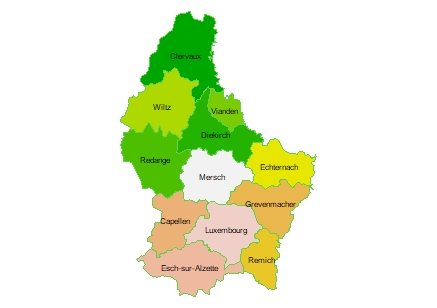
\includegraphics[scale=0.6]{Lux_map3.jpeg}
\end{figure}
\end{frame}


\begin{frame} [fragile]
\begin{tiny}
\begin{verbatim}
# Contiguity-based neighbours

# Derive the neighbourhood structure from the shapefile using poly2nb function.
# Here rook's move contiguity is used (at least one edge is shared between polygons)
w.rook <- poly2nb(lux, row.names=lux$ID_2, queen=FALSE)

# The nb object w.rook lists for each polygon the neighboring polygons.
# For example, to see the neighbors for the first polygon in the object, type:
w.rook[[1]]

> w.rook[[1]]
[1] 2 4 5

# Check it by plotting Luxembourg with the numerical identifier of the cantons
par(mar=c(0,0,0,0))
plot(lux,border=3, col=terrain.colors(length(lux)), axes=F)
text(lux,"ID_2",cex=1)

\end{verbatim}
\end{tiny}
\vspace{-10pt}
\begin{figure}
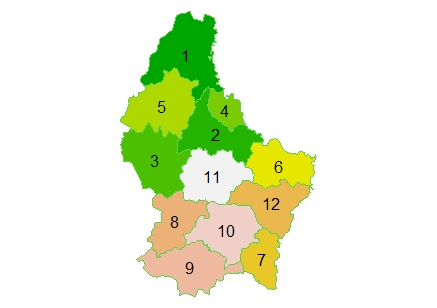
\includegraphics[scale=0.55]{Lux_map.jpeg}
\end{figure}
\end{frame}



\begin{frame} [fragile]
\begin{tiny}
\begin{verbatim}
# Now, assign the weights to each neighboring polygon.
# The argument style can take on a number of character values:
# W=row standardized, B=binary, C=globally standardized
# with zero.policy = TRUE we insert zero into the weights matrix where there is no connection

w.rook.l <- nb2listw(w.rook, style="B", zero.policy=TRUE) # binary (0/1) weights

# Check the weight of the first polygon's three neighbors
w.rook.l$weights[1]

> w.rook.l$weights[1]
[[1]]
[1] 1 1 1

# Inspect also the weight matrix
w.rook.m <- nb2mat(w.rook, style="B", zero.policy = TRUE) #  spatial weights matrix
w.rook.m

# Compute coordinates at centroids of each canton
coords <- coordinates(lux)

# Plot
par(mai=c(0,0,0,0))
plot(lux, col='white', border='blue')
plot(w.rook, coords, col='red', lwd=2, add=TRUE)

\end{verbatim}
\end{tiny}
\end{frame}


\begin{frame} [fragile]
\begin{tiny}
\begin{verbatim}
# Distance-based neighbours

IDs <- row.names(as(lux, "data.frame"))

w.d_k3 <- knn2nb(knearneigh(coords, k=3), row.names = IDs)# 3 nearest neighbours for spatial weights

# Plot
par(mai=c(0,0,0,0))
plot(lux, col='white', border='blue')
plot(w.d_k3, coords, col='red', lwd=1, add=TRUE)

w.d10 <- dnearneigh(coords, 0, 10) # neighbourhood contiguity by distance

# Plot
par(mai=c(0,0,0,0))
plot(lux, col='white', border='blue')
plot(w.d10, coords, col='red', lwd=1, add=TRUE)
\end{verbatim}
\end{tiny}
\vspace{-7pt}
\begin{figure}
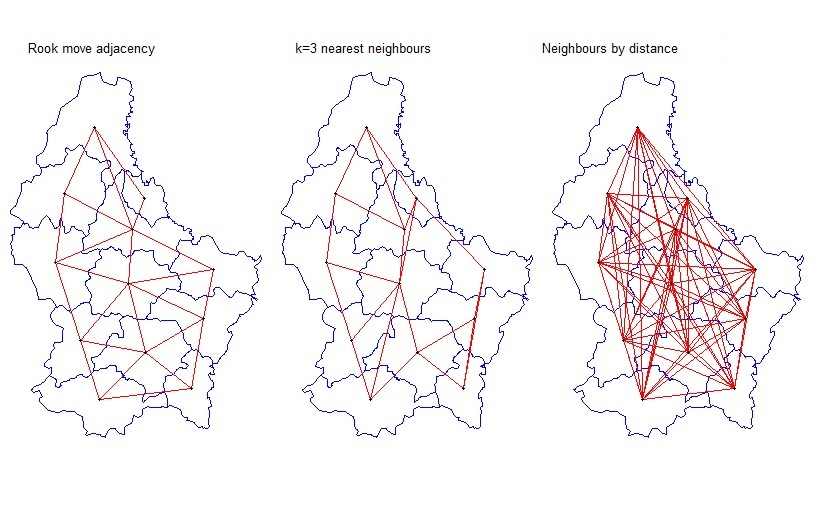
\includegraphics[scale=0.53]{Lux_neigh3.jpg}
%\caption{\footnotesize Plot of three neighbourhood structures}
\end{figure}
\end{frame}

\begin{frame}
\frametitle{References}
\begin{itemize}
\item Haining R., Guangquan L. (2020), Modelling Spatial and Spatial-Temporal Data. A Bayesian Approach, CRC Press, Sections 4.2, 4.3
\item Bivand R., Creating Neighbours, available at: \url{https://r-spatial.github.io/spdep/articles/nb.html}
\end{itemize}
\end{frame}

\end{document} 